\chapter{Analiza tematu wyszukiwania tekstu}  % Analiza tematu
% 

%\begin{itemize}
%\item Jaki problem chcę (muszę :-) rozwiązać?
%\item Dlaczego rozwiązanie problemu jest ważne?
%\item Jak inni rozwiązują ten problem?
%\item Jakie są zalety i wady tych rozwiązań?
%\end{itemize}

%Odwołania do literatury:
%książek \cite{bib:ksiazka},
%artykułów w czasopismach \cite{bib:artykul},
%materiałów konferencyjnych \cite{bib:konferencja}
%i stron www \cite{bib:internet}.
%
%Równania powinny być numerowane
%wzór
%\begin{align}
%    y = \frac{\partial x}{\partial t}
%\end{align}
%
%
%\begin{itemize}
%\item analiza tematu
%\item wprowadzenie do dziedziny (\english{state of the art}) – sformułowanie problemu, 
%\item poszerzone studia literaturowe, przegląd literatury tematu (należy wskazać źródła wszystkich informacji zawartych w pracy)
%\item opis znanych rozwiązań, algorytmów, osadzenie pracy w kontekście
%\item Tytuł rozdziału jest często zbliżony do tematu pracy. 
%\item Rozdział jest wysycony cytowaniami do literatury \cite{bib:artykul,bib:ksiazka,bib:konferencja}. 
%Cytowanie książki \cite{bib:ksiazka}, artykułu w czasopiśmie \cite{bib:artykul}, artykułu konferencyjnego \cite{bib:konferencja} lub strony internetowej \cite{bib:internet}.
%\end{itemize}

%\begin{Definition}\label{def:1}
%Definicja to zdanie (lub układ zdań) odpowiadające na pytanie o strukturze „co to jest a?”. Definicja normalna jest zdaniem złożonym z 2 członów: definiowanego (łac. definiendum) i definiującego (łac. definiens), połączonych spójnikiem definicyjnym („jest to”, „to tyle, co” itp.). 
%\end{Definition}
%
%\begin{Theorem}[Pitagorasa]\label{t:pitagoras}
%W dowolnym trójkącie prostokątnym suma kwadratów długości przyprostokątnych jest równa kwadratowi długości przeciwprostokątnej tego trójkąta. 
%\end{Theorem}
%
%\begin{Example}[generalizacja]\label{ex:generalizacja}
%Przykładem generalizacji jest para: zwierzę i pies. Pies jest zwierzęciem. Pies jest uszczegółowieniem pojęcia zwierzę. Zwierzę jest uogólnieniem pojęcia pies.
%\end{Example}
\section{Sformułowanie problemu}
Wyszukiwanie tekstu w systemach towarzyszy ludziom od początków istnienia maszyn.
Jednak pierwsze komputery nie posiadały ogromnych ilość pamięci. Z biegiem lat
zaistniała potrzeba odkrycia algorytmów wyszukujących zawartość pamięci. 
Procesor Intel 8008 zaprezentowany w 1972 posiadał jedynie 14-bitową magistralę
adresową, co pozwalało na 16 KB pamięci \cite{bib:internet:Intel8008}. 
Obecna ilość pamięci, którą można otrzymać po założeniu konta z chmury Google'a to 15 GB
\cite{bib:internet:GoogleCloud}, co stanowi milion maksymalnych bloków pamięci w 
urządzeniu ze wspomnianym procesorem Intela. Należy zauważyć, że lokalne zasoby
 pamięci znacznie przewyższają te, które możemy otrzymać za darmo w chmurze.

Zasadniczym problem naszej pracy jest wyszukiwanie zawartości tekstowej
ogromnej ilość plików w różnych formatach. Takie podejście może okazać się 
problematyczne \newline w przypadku plików dźwiękowych, filmowych czy zdjęć
wszelkiego rodzaju. Dodatkowym problemem może okazać się rozwiązanie problemu
przeszukiwania zagnieżdżonych w sobie archiwów.

\section{Dostępne rozwiązania} %state of art

Podjęcie problemu wyszukiwania plików po nazwach oraz zawartości jest bardzo
złożonym i trudnym problemem w sferze programistycznej. Istnieje kilka rozwiązań
tego problemu. Narzędzia takie jak \textbf{find}, \textbf{grep} czy \textbf{ripgrep} 
\cite{bib:internet:ripgrep} pozwalają na wyszukiwanie tekstu. Narzędzia te nie 
są przystosowane do znalezienia pełnej ścieżki pliku dla archiwów, a są jedynie
w stanie określić kontekst znalezienia, bez dokładniej ścieżki pliku.

\subsection{Przykładowe narzędzia dostępne do wykorzystania}

Narzędzie \textbf{find} to znane i popularne narzędzie w systemie z jądrem Linux.
Jest ono bardzo często wykorzystywane do znajdowania plików w systemie po nazwie, 
jednak nie jest przystosowane do znajdowania zawartości plików.

\begin{figure}[htbp]
  \centering
\begin{tcolorbox}[
    colback=white,
    colframe=black,
    boxrule=0.5pt,
    arc=0pt
]
  \begin{minted}{bash}
find /biblioteka -name '*.pdf'
find /biblioteka -path 'książki/*.docx' 
find /biblioteka -name '*.py' -not -path '*/site-packages/*'  
find /biblioteka -maxdepth 2 -size +500k -size -10M           
find /biblioteka -type f -empty -delete 
  \end{minted}
\end{tcolorbox}
\caption{Przykład użycia programu find}
\label{fig:cmd:findExamples}
\end{figure}

Jak pokazano na rysunku (rys. \ref{fig:cmd:findExamples}) te przykładowe komendy find
pozwalają na wyszukanie zawartości folderu biblioteka, a kolejne argumenty 
pozwalają na doprecyzowanie określonych parametrów pliku. Argument \textbf{-name}
pozwala na wyszukanie wszystkich słów odpowiadających nazwie pliku, jednak nie
uwzględniają ścieżki. Argument \textbf{-path} pozwala na wyszukanie plików, 
które odpowiadają podanej ścieżce, a nie jedynie nazwie pliku.

Połączenie argumentów \textbf{-name} oraz argumentu \textbf{-not} z \textbf{-path}
umożliwi wyszukanie plików z rozszerzeniem .py. Dodatkowo odrzucone zostaną 
pliki z paczek pobocznych (ang. \english{site-packages}).

Kolejna komenda wyszuka wszystkie pliki znajdujące się tylko w folderze 
/biblioteka (\textbf{-maxdepth 2}) oraz jednym zagnieżdżonym folderze poniżej.
Dodatkowo pokazane zostaną pliki większe niż 500 KB i mniejsze niż 10 MB.

Ostatnia komenda z rysunku (rys. \ref{fig:cmd:findExamples}) daje możliwość usunięcia 
(\textbf{-delete}) plików (nie folderów) \textbf{-type f}, które są puste (\textbf{-empty}).

Narzędzie to niestety nie ma możliwości przeszukania folderów z pliku
archiwum. Aby dokonać takiego przeszukania, należy wykonać dekompresję danych
przy użyciu tar lub innego podobnego narzędzia. Taki proces nie jest jednak 
prosty w przypadku wielu typów archiwów.

Do przeszukiwania zawartości plików dobrze nadaje się narzędzie grep, które jest
dostępny ogólnodostępnym narzędziem GNU (skrót \ref{skrót:GNU}). Jego działanie jest dość podobne do \textbf{find'a},
gdyż posiada on możliwość wyszukiwania treść w plikach tekstowych. Grep również nie 
posiada też możliwość szukania zawartości archiwów oraz nie wspiera wielu 
formatów. Jest możliwość binarnego przeszukania plików, lecz archiwa nie będą 
odczytane w przypadku użycia kompresji.

\begin{figure}[htbp]
  \centering
\begin{tcolorbox}[
    colback=white,
    colframe=black,
    boxrule=0.5pt,
    arc=0pt
]
  \begin{minted}{bash}
grep "szukany-tekst" /biblioteka/plik1.txt 
grep -r "szukany-tekst" /biblioteka 
grep -i "szukany-tekst" /biblioteka/plik1.txt
grep -w "szukany-tekst" /biblioteka/plik1.txt
grep -C 2 "szukany-tekst" plik1.txt
cat /biblioteka/plik1.txt | grep -v "szukany-tekst" 
  \end{minted}
\end{tcolorbox}
\caption{Przykład użycia programu grep}
\label{fig:cmd:grepExamples}
\end{figure}

Na rysunku powyżej przedstawione są przykładowe komendy programu grep 
(rys. \ref{fig:cmd:grepExamples}). Pierwsza komenda wyszukuje tekst 'szukany-tekst' w pliku /biblioteka/plik1.txt.
Kolejna komenda pozwala nam przeszukać rekurencyjnie wszystkie pliki w folderach znajdujące się w 
/biblioteka (\textbf{-r}). Trzecia komenda wyszuka wszystkie wystąpienia 
'szukany-tekst' ignorując przy tym wielkość liter. To pozwoli wyszukać tekst
posiadający treść 'szukany-tekst' w pliku. Dodając argument \textbf{-w}
wyświetla się liczba wiersza, w którym znajdowało się dopasowanie w pliku. 

Przedostatnia komenda pozwala na pokazanie kontekstu znalezionego dopasowania 
(rys. \ref{fig:cmd:grepExamples}). Jeżeli 'szukany-tekst' znajduje się w linii 25, to
program przedstawi nam linie od 23 do 27 z wyszczególnioną treścią, którą 
wyszukiwano. Ostatnia komenda przyjmuje treść innego programu przy pomocy
standardowego wejścia strumieniowego. Ta komenda zwróci nam wszystkie linie,
w których 'szukany-tekst' nie występuje.

Kolejnym narzędziem jest \textbf{ripgrep}. Nie jest on domyślnie instalowany na 
większości systemów Linux, ale pozwala na szybsze wyszukiwanie z powodu
wykorzystania równoległości wątków.

\begin{figure}[htbp]
  \centering
\begin{tcolorbox}[
    colback=white,
    colframe=black,
    boxrule=0.5pt,
    arc=0pt
]
  \begin{minted}{bash}
rg "szukany-tekst" /biblioteka
rg -i "szukany-tekst" /biblioteka
rg -l "szukany-tekst" /biblioteka
rg -c "szukany-tekst" /biblioteka
rg -U "szukany\ntekst" /biblioteka
rg -z "szukany-tekst" /biblioteka/archiwum.zip
  \end{minted}
\end{tcolorbox}
\caption{Przykład użycia programu ripgrep}
\label{fig:cmd:ripgrepExamples}
\end{figure}

Przykładowa komenda pozwalające na wyszukanie frazy 'szukany-tekst' we wszystkich
folderach i podfolderach /biblioteka (rys. \ref{fig:cmd:ripgrepExamples}). Kolejna
komenda pozwala na wyszukanie wszystkich fraz z pominięciem wielkości znaków. 
Podając parametr \textbf{-l} otrzymano nazwy plików bez linii, w których 
wystąpiła fraza. Parametr \textbf{-c} zwróci nam ilość wystąpień tego wyrazu w 
pliku. Parametr \textbf{-U} pozwala na znalezienie wzorca występującego przez 
kilka linii. Parametr \textbf{-z} pozwala na przejrzenie nierozpakowanego 
archiwum. Ostatnia opcja jest bardzo dobra dla plików, które znajdują się w 
zbiorze danych.

\section{Odniesienia do literatury}

Istnieje wiele odniesień do wyszukiwania danych w literaturze. Praca Google 
\cite{bib:internet:htmlSearchGoogle} odnosi się do problemu wyszukiwania tekstu 
w dobie internetu i ilości danych, która jest przechowywana w chmurze. 
Indeksowanie stron przyspiesza wyszukiwanie, ale wymaga dodatkowej przestrzeni
pamięci na przechowywanie zaindeksowanych danych.

Ilość wydobywanych i dostarczanych danych poprzez operacje wejścia i wyjścia stanowi duże wyzwanie
oraz wymaga wykorzystania skomplikowanych algorytmów i jest skomplikowanym
problemem. 

Operacje wejścia-wyjścia (I/O) stanowią kluczowy element w architekturze 
komputerowej, wpływając na ogólną wydajność systemu. W artykule 'W skrócie o 
wydajności pamięci' porównano zarządzanie danymi w komputerze do 
organizacji przedmiotów w domu, podkreślając znaczenie efektywnego 
rozmieszczenia i dostępu do zasobów. W kontekście operacji I/O analogie do 
fizycznych obiektów pomagają zrozumieć, jak istotne jest minimalizowanie 
opóźnień \cite{bib:internet:IntelMemoryPerformance}. 

Jednym z głównych wyzwań w operacjach I/O jest różnorodność i zmienność 
urządzeń peryferyjnych. Urządzenia te różnią się pod względem szybkości 
działania, protokołów komunikacyjnych oraz sposobu obsługi przez system 
operacyjny. W notatkach dotyczących systemów operacyjnych zwraca się uwagę na 
problem identyfikacji źródła przerwania. Konieczność obsługi współbieżnej 
wielu urządzeń komplikuje proces zarządzania operacjami I/O co opisane
zostało na wykładzie \cite{bib:internet:UrzadzeniaWejsciaWyjscia}. 

Kolejnym istotnym aspektem jest zarządzanie pamięcią podręczną (cache) w 
kontekście operacji I/O. Efektywne wykorzystanie pamięci cache może znacząco 
zmniejszyć opóźnienia dostępu do danych, jednak wymaga to zaawansowanych 
mechanizmów koherencji, zwłaszcza w systemach wieloprocesorowych. W artykule 
'W skrócie o wydajności pamięci' omówiono hierarchię pamięci oraz znaczenie 
odpowiedniego rozmieszczenia danych w celu optymalizacji wydajności \cite{bib:internet:IntelMemoryPerformance}.

Na ten temat w swojej pracy doktorskiej odniósł się też dr Artur Malinowski \cite{bib:internet:ArturMalinowskiIO}.
W tej pracy do złożoności systemów odzyskiwania danych (str. 24). Dane 
przetrzymywane w określonym obszarze pamięci L1, L2, L3 znajdują się
bliżej niż na dysku SSD lub HDD i przez to zostaną znacznie szybciej odszukane. 

Artykuł 'Love your cache' \cite{bib:internet:TwojaPamiećPodręczna} przedstawia
kompleksowe podejście do zarządzania 
pamięcią podręczną w kontekście nowoczesnych aplikacji internetowych. Przede 
wszystkim, artykuł podkreśla znaczenie strategicznego podejścia do buforowania 
treści w pamięci podręcznej przeglądarki. Autor wskazuje, że standardy 
dotyczące pamięci podręcznej pochodzące z 1999 roku nie są w pełni dostosowane 
do współczesnych wymagań aplikacji internetowych. Proponowane jest wprowadzenie
bardziej zaawansowanych mechanizmów kontroli, które pozwalają na optymalizację
wydajności przy jednoczesnym zachowaniu aktualności danych.

Istotnym elementem omawianym w artykule jest koncepcja odcisków cyfrowych w
nazwach plików. Polega ona na dodawaniu unikalnych identyfikatorów do nazw 
zasobów, co umożliwia efektywne zarządzanie przechowywanym danymi w pamięci 
podręcznej. Jest to szczególnie ważne w kontekście optymalizacji wydajności.

Podczas konferencji TREC \cite{bib:konferencja:TRECDuplicates} jeden z zespołów 
napotkał problem zduplikowanych danych. Chęć wydobycia danych w celu utworzenia
tekstów wymagało usunięcia duplikacji dokumentów oraz wyborze tej treści,
która posiada najwięcej wartości. Mogłoby to być tematem rozszerzenie pracy. 

Archiwizacja danych stanowi istotne wyzwanie w różnych dziedzinach, od medycyny 
po zarządzanie dokumentami historycznymi. Analiza systemów archiwizacji obrazów
medycznych oraz procesów ekstrakcji piśmiennictwa wskazuje na kluczowe problemy
i rozwiązania stosowane w tych obszarach. W dokumencie o technicznej formie
proponowanych rozwiązań problemów można w 'Przegląd otwartych rozwiązań systemów 
archiwizacji i komunikacji obrazów medycznych' \cite{bib:internet:ArchiwizacjaDanychMedycznych}.

Archiwa przechowywane mogą też być w różnym stanie. Niektóre dane mogą być
uszkodzone z powodu złego przechowywania, sposobu pozyskanych danych lub 
niepoprawnej implementacji odczytu danych z archiwów. W rządowym artykule o
digitalizacji piśmiennictwa można znaleźć analogię do rozwiązywanego problemu \cite{bib:internet:GovDigitalizacjaPiśmiennictwa}.

Dodatkowym problemem odczytywanie dużych zarchiwizowanych danych. W książce W.
Curtis Prestona można przeczytać o problemie odczytania tych danych w przypadku
uszkodzonych zawartości \cite{bib:ksiazka:ArchiwizacjaIOdzyskiwanie}. Sugeruje
on wiele narzędzi pozwalających na odzyskanie zawartości z archiwów i problem
z radzeniem sobie w przypadkach uszkodzenia danych.

Problemem odczytywania danych mocno skompresowanych, zajmowali się również 
doktorzy z Uniwersytetu w Dublinie \cite{bib:internet:KompresjaDanych}. Odnosili
się oni do skomplikowania odczytu i redundancji w przypadku transportu danych
przez sieć.

\section{Opis poznanych rozwiązań}

\subsection{Algorytm brute force}

\begin{figure}[htbp]
  \centering
  \begin{lstlisting}
for i := 0; i<len(pattern); i++{
  for j := 0; j<len(substring); j++{
    // compare bytes
  }
}
  \end{lstlisting}
  \caption{Przykład algorytmu brute force}
  \label{fig:code:bruteForceComparison}
\end{figure}

Jest wiele algorytmów, które wyszukują tekst. Jednym z takich algorytmów, jest 
algorytm typu brute-force. Polega na sprawdzaniu każdego bajtu, a jego implementacja
jest traktowana jako naiwna. Złożoność czasowa tego rozwiązania wynosi
$O(len(pattern) * len(substring))$, gdzie len(pattern) to długość bloku 
przeszukiwanego, a len(substring) to długość tekstu szukanego. Nie jest wykonana
żadna optymalizacja w tym algorytmie, jak np. przesunięcie się do następnej
 instancji znaku powtórzonego. Przykładową implementację algorytmu można znaleźć
  na rysunku (rys. \ref{fig:code:bruteForceComparison}).

%\begin{figure}[htbp]
%  \centering
%  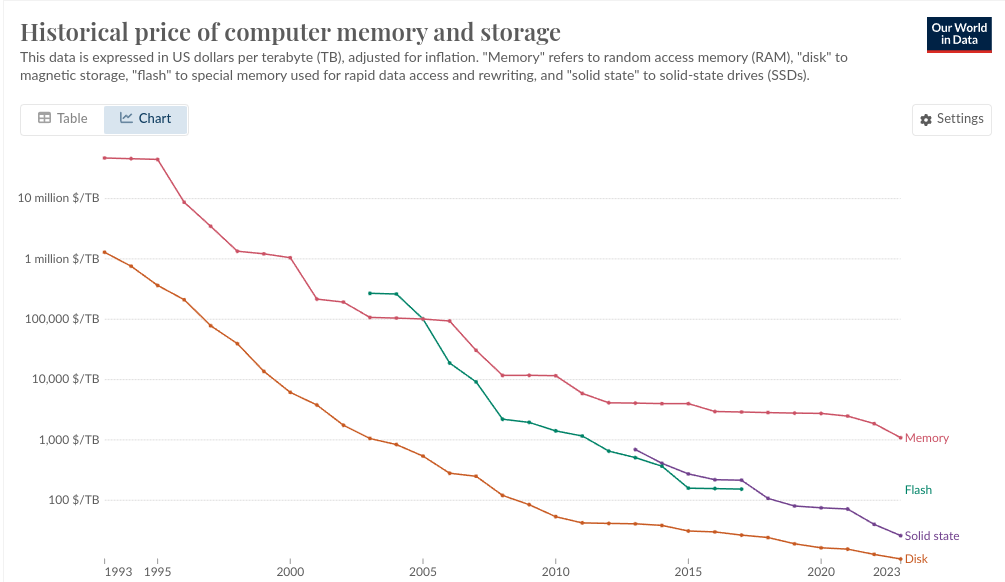
\includegraphics[width=0.9\textwidth]{./images/historical-mem-price.png}
%  \caption{Historyczne dane cen pamięci w latach 1993-2023}
%  \label{screenshot:MemPrices}
%\end{figure}
%\cite{internet:HistoricalMemPrice}
%https://jcmit.net/memoryprice.htm

\subsection{Algorytm Morisa-Pratta}

\begin{figure}[htbp]
  \centering
  \begin{lstlisting}
preproc := make([]byte, len(substr)+1)
curr = -1
preproc[0] = -1
for i := 1; i <= len(substr); i++ {
  for (curr > -1) && (substr[curr] != substr[i-1]) {
    curr = preproc[curr]
  }
  curr++
  preproc[i] = curr
}
  \end{lstlisting}
  \caption{Przykład uprzedniego procesowania tekstu szukanego}
  \label{fig:code:preprocessMorisPratt}
\end{figure}

Algorytm Morisa-Pratta, jest algorytmem wykorzystującym możliwość procesowania 
łańcucha w tekście, aby dopasować wcześniej odpowiadającą część zbioru
(rys. \ref{fig:code:preprocessMorisPratt}). Polega on na wykorzystaniu faktu
 istnienia pasującego prefikso-sufiksu. Pozwala on na pominięcie porównania
 znaków, które się powtarzają w łańcuchu poszukiwanym.

Dzięki wykorzystaniu tej zależności można uniknąć cofania się indeksu i. 
Od teraz jako tablicę przechowującą informacje o przesunięciu w przypadku 
błędnego znaku, którą zainicjowano na rysunku (rys. \ref{fig:code:preprocessMorisPratt})
jako tablica \textbf{preproc}.

\begin{figure}[htbp]
    \centering
    \begin{lstlisting}
  res := []int{}
  curr := 0
  found := 0
  for i := 0; i < len(pattern); i++ {
    for (curr > -1) && (substr[curr] != pattern[i]) {
      curr = preproc[curr]
    }
    curr++
    if curr == len(substr) {
      for found < i-curr+1 {
        found++
      }
      res = append(res, found)
      found++
      curr = preproc[curr]
    }
  }
    \end{lstlisting}
    \caption{Przykład procesowania łańcucha poszukiwanego w algorytmie Morisa Pratta}
    \label{fig:code:algoMorisPratt}
  \end{figure}

Tablice \textbf{preproc} należy wypełnić poprzednią wartości tak długo, aż zaistnieje
różnica pomiędzy obecnym, a następnym znakiem tablicy szukanej (tablicy 
\textbf{substr}). W przypadku różnicy obu znaków — zwiększa się wartość zapisywaną 
do tablicy \textbf{preproc} o odległość różnicy znaków. W ten sposób następnym
 razem będzie możliwość pominięcia porównania tych znaków.

W drugim etapie można wykorzystać wcześniej przygotowaną tablice przemieszczeń 
\textbf{preproc}, aby obliczyć ilość przesunięcia w przypadku znalezienia 
niepasującego prefiksu (rys. \ref{fig:code:algoMorisPratt}). Dzięki temu zwykle 
dłuższy tekst znajdujący się we wzorcu \textbf{pattern} można przeanalizować szybciej
niż w przypadku algorytmu brute-force.

\begin{figure}[htbp]
    \centering
\begin{lstlisting}
func Index(pattern, substr string) int {
  n := len(substr)
  switch {
  case n == 0:
    return 0
  [...]
  case n > len(pattern):
    return -1
  case n <= bytealg.MaxLen: // Zwykle ten przypadek uzyty
    // brute-force kiedy pattern jest krotki
    if len(pattern) <= bytealg.MaxBruteForce /* max == 64 */{
      return bytealg.IndexString(pattern, substr)
  }
  [...]
  }
}
\end{lstlisting}
\caption{Szukanie łańcucha w standardowej bibliotece Golang}
\label{fig:code:golangSearchInsideString}
\end{figure}
W podstawowej bibliotece języka Golang, w pakiecie \textit{strings} istnieje 
implementacja metody \textit{Index()}. Nie jest ona jednak w pełni przedstawiona
w kodzie, natomiast w jej implementacji można zauważyć, że algorytm brute-force
jest wykorzystywany tylko w przypadku, gdy długość wzorca wynosi więcej niż 64 
(rys. \ref{fig:code:golangSearchInsideString}).

W implementacji wyszukiwania w Golang, gdy bufor szukany jest mniejszy niż 64 bajty,
obliczenie bufora wcześniejszego procesowania \textbf{BWP} nie jest wykonywane, 
wiec stosuje się algorytm brute-force. Jeżeli wzorzec jest większy niż 64 
bajty to wykonuje się wyszukanie z pomocą \textbf{BWP}.

W Golang, gdy wzorzec jest większy niż
64 znaki, to wykonuje się inny algorytm, który posiada dodatkową walidację w
przypadku odkrycia wyniku fałszywie dodatniego. Algorytm Morisa-Pratta nie
 potrzebuje takiej walidacji.

\subsection{Algorytm Kurta-Morisa-Pratta}

\begin{listing}[H]
    \begin{minted}[xleftmargin=0.15\textwidth,xrightmargin=0.2\textwidth,linenos]{diff}
preproc := make([]int, lensubstr+1)
preproc[0] = -1
curr := -1
for i := 1; i <= lensubstr; i++ {
  for (curr > -1) && (substr[curr] != substr[i-1]) {
    curr = preproc[curr]
  }
  curr++
- preproc[i] = curr
+ if (i == lensubstr) || (substr[i] != substr[curr]) {
+   preproc[i] = curr
+ } else {
+   preproc[i] = preproc[curr]
+ }
}
mp.preproc = preproc
    \end{minted}
  \caption{Różnica pomiędzy algorytmami KMP i MP}
  \label{fig:code:KurtMorisPrattVsMorisPratt}
\end{listing}

Kolejny rozpatrywany algorytm jest implementacja, rozszerzająca poprzednią 
implementację przedstawioną w algorytmie Morisa-Pratta. Różnice można zauważyć na podstawie rysunku
(rys. \ref{fig:code:KurtMorisPrattVsMorisPratt}).

Gdy nie osiągnięto długości łańcucha i obecny znak jest równy temu, który 
znajduje się w łańcuchu szukanym (rys. \ref{fig:code:KurtMorisPrattVsMorisPratt}
linijka 10), to można wykonać skok do znaku znajdującego się w tablicy
przygotowanej (rys. \ref{fig:code:KurtMorisPrattVsMorisPratt} linijka 13).
Nie należy sprawdzać kolejnego znak w pętli. Ta różnica powoduje, że algorytm 
wykonuje się szybciej.

Złożoność tego algorytmu wynosi $O(2*{len(pattern)})$, gdzie pattern to długość
tekstu przeszukiwanego. W najbardziej pesymistycznym przypadku, gdy nie 
znaleziono dopasowania, będzie to wymagało ilości operacji powrotu równej długości 
łańcucha szukanego. Powoduje to, że złożoność obliczeniowa sprowadza się do
$O({len(substr)}*{len(pattern)})$, co posiada tę samą złożoność co algorytm naiwny. 

\begin{table}[hbtp]
  \centering
  \begin{tabular}{ |c|c|  } 
    % \hline
    % \multicolumn{2}{|c|}{Przykład wykorzystania algorytmu KMP} \\
    \hline
    wzorzec S & AAAAAABAAAAAABAAAAAAA \\
    \hline
    łańcuch W & AAAAAA \\
    \hline
    liczba cofnięć & 20 \\
    \hline
  \end{tabular}
  \caption{Przykład wykorzystania algorytmu KMP}
  \label{tabela:KMPExampleSlow}
\end{table}

W scenariuszu wykorzystania algorytmu Kurta-Morrisa-Pratt (tab. \ref{tabela:KMPExampleSlow})
można zaobserwować działanie na przykładzie tekstu przeszukiwanego S = 
'AAAAAABAAAAAABAAAAAAA' oraz frazy szukanej W = 'AAAAAA'. W tym przypadku algorytm musi sprawdzić każde
wystąpienie 'A' przed dotarciem do 'B', co jest bardzo nieefektywne, ponieważ
pisany tekst miałby większą różnorodność liter i proces przeszukiwania mógłby 
zacząć się od symbolu B. Sytuacja 
pogarsza się wraz ze wzrostem liczby powtórzeń fragmentu "AAAAAAB". Mimo że 
metoda tablicowa \textbf{preproc} działa tu sprawnie (bez potrzeby cofania się), to jej 
jednokrotne wykonanie dla łańcucha szukanego W wykona się podobnie jak w algorytmie
brute-force. Proces ten wyszukiwania często wymaga wielokrotnych powtórzonych przebiegów. 
Wielokrotne przeszukiwanie tekstu S w poszukiwaniu wzorca prowadzi do gorszej
wydajności, gdy zbiór danych zawiera tego typu 
charakterystykę tekstu i wzorca (powtarzające się litery). Naturalny język posiada
rzadziej powtarzające się litery, dlatego algorytm Boyera-Moore'a może stanowić 
optymalne rozwiązanie.

Algorytm KMP wykorzystuje w najgorszym przypadku liniowy przebieg, natomiast
algorytm Boyera-Moore'a w najlepszym przypadku posiada złożoność $O({len(pattern)}+{len(substr)})$, a w 
najgorszym przypadku $O({len(pattern)}*{len(substr)})$.

\subsection{Algorytm Boyera-Moore'a}
\label{sch:algoBoyerMoore}

\begin{figure}[htbp]
    \centering
    \begin{lstlisting}
i := 0
len_str := len(str)
len_substr := len(substr)
for i+len_substr <= len_str {
  for j := len_substr - 1; j >= 0; j-- {
   if str[i+j] != substr[j] {
     if loc := bm.preproc[str[i+j]]; loc == 0 {
       if j == len_substr-1 {
         i += len_substr
       } else {
         i += len_substr - j - 1
       }
     } else {
       n := loc - len_substr + j + 1
       if n <= 0 {
         i++
       } else {
         i += n
       }
     }
     goto loop
   }
  }
  res = append(res, i)
  if v := bm.preproc[str[i+len_substr-1]]; v != 0 {
   i += v
  } else {
   i += len_substr
  }
}
    \end{lstlisting}
    \caption{Główna część wyszukiwania w algorytmie Boyera-Moore'a}
    \label{fig:code:BMmain}
\end{figure}

Algorytm Boyera-Moore'a wprowadza rewolucyjne podejście poprzez skanowanie 
wzorca od prawej do lewej strony, w przeciwieństwie do MP i KMP, które 
analizują tekst od lewej do prawej. Ta fundamentalna różnica pozwala algorytmowi BM na 
znacznie efektywniejsze przeskakiwanie fragmentów tekstu (rys. \ref{fig:code:BMmain}), które na pewno nie 
zawierają wzorca. BM wykorzystuje dwie heurystyki: "złego znaku" oraz "dobrego
sufiksu", podczas gdy KMP i MP opierają się na pojedynczej tablicy prefiksowej.

Zaletą algorytmu jest to, że ilość skoków pomiędzy porównaniami jest zwykle 
większa od 1, a gdy istnieje sytuacja, w której litery w łańcuchu szukanym nie
powtarzają się, to można przeskoczyć o długość całego łańcucha szukanego.

\begin{figure}[htbp]
    \centering
    \begin{lstlisting}
if bm.preproc == nil {
  l := len(substr)
  table := make([]int, 256)

  for i := 0; i < l-1; i++ {
    j := substr[i]
    table[j] = l - i - 1
  }
  bm.preproc = table
}
    \end{lstlisting}
    \caption{Kalkulacja BWP w algorytmie Boyera-Moore'a}
    \label{fig:code:BMpreproc}
\end{figure}

W kontekście implementacji algorytm Boyera-Moore'a wymaga utworzenia tokenów dla
każdego znaku w ASCII (rys. \ref{fig:code:BMpreproc}) w buforze wcześniejszego 
procesowania (skrót \ref{skrót:BWP}), co zwiększa złożoność pamięciową w porównaniu do pojedynczej 
tablicy prefiksowej w KMP i MP. Jednak ta dodatkowa pamięć przekłada się na 
możliwość wykonywania większych skoków w tekście. KMP i MP różnią się między 
sobą głównie w sposobie konstrukcji tablicy prefiksowej. KMP wykorzystuje 
bardziej zaawansowaną technikę, która pozwala na uniknięcie niektórych 
niepotrzebnych porównań występujących w MP.

Praktyczny wybór między tymi algorytmami zależy od charakterystyki danych
wejściowych. BM sprawdza się najlepiej w przypadku długich wzorców i tekstów
napisanych w językach naturalnych, gdzie występuje duża różnorodność znaków.
KMP i MP są bardziej przewidywalne w działaniu i mogą być lepszym wyborem dla 
krótkich wzorców lub tekstów o ograniczonym alfabecie jak na przykład sekwencje
DNA.

Z tego też powodu należy wykonać heurystykę danych, które są analizowane.
Można to zrobić na kilka sposobów i zostanie to przedstawione w następnych rozdziałach.
